
%(BEGIN_QUESTION)
% Copyright 2010, Tony R. Kuphaldt, released under the Creative Commons Attribution License (v 1.0)
% This means you may do almost anything with this work of mine, so long as you give me proper credit

Read and outline the ``Contacts and Coils'' subsection of the ``Ladder Diagram (LD) Programming'' section of the ``Programmable Logic Controllers'' chapter in your {\it Lessons In Industrial Instrumentation} textbook.  Note the page numbers where important illustrations, photographs, equations, tables, and other relevant details are found.  Prepare to thoughtfully discuss with your instructor and classmates the concepts and examples explored in this reading.

\vskip 20pt \vbox{\hrule \hbox{\strut \vrule{} {\bf Suggestions for Socratic discussion} \vrule} \hrule}

\begin{itemize}
\item{} If you have access to your own PLC for experimentation, I urge you to write a simple {\it demonstration} program in your PLC allowing you to explore the behavior of these PLC instructions.  The program doesn't have to do anything useful, but merely demonstrate what each instruction does.  First, read the appropriate section in your PLC's manual or instruction reference to identify the proper syntax for that instruction (e.g. which types of data it uses, what address ranges are appropriate), then write the simplest program you can think of to demonstrate that function in isolation.  Download this program to your PLC, then run it and observe how it functions ``live'' by noting the color highlighting in your editing program's display and/or the numerical values manipulated by each instruction.  After ``playing'' with your demonstration program and observing its behavior, write comments for each rung of your program explaining in your own words what each instruction does.
\end{itemize}

\underbar{file i04517}
%(END_QUESTION)





%(BEGIN_ANSWER)

\noindent
{\bf Demonstration program showing some basic bit instructions in an Allen-Bradley MicroLogix PLC:}

$$\includegraphics[width=15.5cm]{i04517x01.eps}$$

Note: your own demonstration program should contain some {\it retentive} coil instruction as well, in order for you to be able to observe what these instructions do and how their operation differs from that of ``regular'' coil instructions!

%(END_ANSWER)





%(BEGIN_NOTES)

Contacts and coils in a Ladder Diagram PLC program are instructions to the PLC's processor to {\it read} and {\it write} discrete data, respectively.  These instructions must be referenced to locations in the PLC's memory.  We may refer to I/O memory registers by hardware location references, or by symbolic addresses where we get to name each input and output according to its real-world function.

\vskip 10pt

Series-connected contacts perform an AND function, while parallel-connected contacts form an OR function.

\vskip 10pt

Two-out-of-Three (2oo3) flame sensor program example.  Motor starter control program example.

\vskip 10pt

It is perfectly okay to use a contact instruction on an output memory bit, since a contact is nothing more than a command for the PLC to {\it read} that bit in memory.  What would be odd is to try to associate a coil ({\it wrote} instruction) with an input bit.

\vskip 10pt

PLCs scan their Ladder Diagrams from left to right, top to bottom, like reading English on a page.  All inputs to a function must be evaluated by the PLC before setting the output status.

\vskip 10pt

``Fail safe'' motor control requires that the Stop pushbutton be physically wired normally-closed (NC), with its corresponding program contact drawn as normally-open (NO).  The NO contact instruction will be typically colored, because the NC Stop pushbutton is typically unpressed and therefore typically sending power to the input of the PLC (thus setting that bit to 1 and actuating the virtual contact in the program).

\vskip 10pt

Another ``fail safe'' feature is to wire an auxiliary contact to its own input on the PLC, then use that input bit to seal-in the logic.  This way, if anything happens in the physical circuit to de-energize the contactor (e.g. an OL tripping, a wire coming loose), the PLC program will unlatch and stop trying to energize the contactor.  This way, when the problem is fixed the motor won't immediately start up again, but rather will wait until the operator presses the ``Start'' button.

\vskip 10pt

Retentive coil instructions (Set and Reset) write to their memory bits when colored, but do nothing when uncolored, allowing the bit to latch in its last state.  These may be used to make a motor start/stop program without using a seal-in contact for latching.  While multiple coil (write) instructions bearing the same address is typically a bad idea, it's necessary when the coils in question are retentive.

PLCs typically energize their real-world outputs at the very end of the program scan, so only that {\it last} bit states written to memory will be sent to the real outputs.  This is important when considering the effects of multiple coil instructions addressed to the same bit, all colored.  Multiple contact instructions with the same address are perfectly okay, because there will be no memory conflict by reading multiple times.

\vskip 10pt

Transition-sensing contact instructions are like {\it one-shot} monostable multivibrator circuits: they act for one scan of the program only, either on a positive transition (from 0 to a 1) or on a negative transition (from 1 to a 0).  PLC scan times are typically in the millisecond range.














\filbreak

\vskip 20pt \vbox{\hrule \hbox{\strut \vrule{} {\bf Suggestions for Socratic discussion} \vrule} \hrule}

\begin{itemize}
\item{} Explain how the 2oo3 flame detection system shown in the book works.
\item{} Explain how you could alter this 2oo3 flame detection system to make it a 1oo3 detection system instead (requiring only one sensor to detect flame in order to energize the lamp).
\item{} Explain how you could alter this 2oo3 flame detection system to make it a 3oo3 detection system instead (requiring all three sensors to detect flame in order to energize the lamp).
\item{} Explain how you could alter this 2oo3 flame detection system to equip it with one more output, indicating if {\it any} of the three sensors failed to detect a flame (as a maintenance alert).
\item{} Explain why the stop pushbutton in the ``fail-stop'' motor control system shown in the book is wired normally-closed (NC) instead of normally-open (NO), and how the PLC program's corresponding virtual contact complements the real-life switch.
\item{} Identify the misconception in this statement: {\it ``PLC contact instructions are always associated with discrete inputs and PLC output instructions always with discrete outputs.''}
\item{} Explain why the final version of this motor control system connects an auxiliary contact from the starter to an input on the PLC, using that as the seal-in rather than an internal bit in the PLC's memory as the seal-in.
\item{} Explain how retentive (latching) coil instructions behave differently from non-retentive coil instructions.
\item{} What happens in a PLC if identically-addressed coils are activated such that they attempt to write conflicting bit states to the same address?
\item{} If you have access to your own PLC for experimentation, demonstrate the function of retentive coil instructions in your own ``demonstration'' program.
\item{} Explain how a ``transition-sensing'' PLC contact instruction works, and why we might wish to use one.
\end{itemize}












\vfil \eject

\noindent
{\bf Prep Quiz:}

The reason most motor control PLC systems use a {\it normally-closed} ``Stop'' pushbutton switch combined with a corresponding {\it normally-open} contact instruction in the program is so that:

\begin{itemize}
\item{} The PLC program will be easier for a technician to understand and diagnose
\vskip 5pt 
\item{} Any ``open'' wiring fault in the Stop pushbutton circuit will keep the motor running
\vskip 5pt 
\item{} The system will be less likely to fail, resulting in less down-time
\vskip 5pt 
\item{} Any ``shorted'' wiring fault will not result in an unsafe operating condition
\vskip 5pt 
\item{} Any ``open'' wiring fault in the Stop pushbutton circuit will stop the motor
\vskip 5pt 
\item{} The motor control will successfully ``seal in'' and latch when started up
\end{itemize}







\vfil \eject

\noindent
{\bf Prep Quiz:}

The purpose of wiring an auxiliary contact on a motor contactor to one if the input channels of a PLC controlling that motor, and using that auxiliary contact signal as a ``seal-in'' is to ensure:

\begin{itemize}
\item{} There will never be a condition when multiple coils in the program conflict with each other
\vskip 5pt 
\item{} Any ``open'' wiring fault in the Stop pushbutton circuit will keep the motor running 
\vskip 5pt 
\item{} Any ``open'' wiring fault in the Stop pushbutton circuit will immediately stop the motor
\vskip 5pt 
\item{} The PLC's output will remain ``on'' even if the motor loses three-phase electrical power
\vskip 5pt 
\item{} The ``forward'' and ``reverse'' contactors may never be simultaneously energized by the PLC
\vskip 5pt 
\item{} The PLC's output will not latch ``on'' if the contactor fails to energize for any reason
\end{itemize}








\vfil \eject

\noindent
{\bf Prep Quiz:}

The purpose of a {\it retentive} coil instruction is to:

\begin{itemize}
\item{} ``Remember'' the last state of the overload contact in a motor control program
\vskip 5pt 
\item{} Write a bit state when activated, and allow that bit to remain latched when not
\vskip 5pt 
\item{} Prevent the possibility of two coil instructions writing to the same address
\vskip 5pt 
\item{} Always write to a bit in memory, whether activated or not by ``virtual power''
\vskip 5pt 
\item{} Permit multiple contact instructions to reference the exact same bit in memory
\vskip 5pt 
\item{} Provide a way to ``reset'' an abnormal fault code in the PLC's memory
\end{itemize}


%INDEX% Reading assignment: Lessons In Industrial Instrumentation, Programmable Logic Controllers (contact and coil programming)

%(END_NOTES)

